\documentclass[10pt]{beamer}

\setbeamertemplate{footline}[page number]

\usepackage{multirow}
\usepackage{stmaryrd}

\theoremstyle{definition}
\newtheorem{answer}{Answer}
\newtheorem{conjecture}{Conjecture}
\newtheorem{question}{Question}

\title{Can we solve Diophantine equations?}

\author{David Ang}

\institute{University College London}

\date{Wednesday, 28 May 2025}

\begin{document}

\frame{\titlepage}

\begin{frame}[t]{Can you solve this?}

\begin{center}
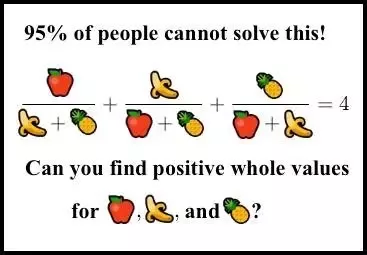
\includegraphics[width=0.7\textwidth]{positive_whole_values.png}
\end{center}

\begin{center}
Smallest positive whole values:

\scriptsize \vspace{0.3cm}

154476802108746166441951315019919837485664325669565431700026634898253202035277999

\vspace{0.1cm}

36875131794129999827197811565225474825492979968971970996283137471637224634055579

\vspace{0.1cm}

4373612677928697257861252602371390152816537558161613618621437993378423467772036
\end{center}

\end{frame}

\begin{frame}[t]{Diophantine equations}

\begin{columns}[T]

\begin{column}{0.8\textwidth}
A \textbf{Diophantine equation}, named after Diophantus of Alexandria, is a \emph{polynomial} equation with \emph{integer} coefficients in \emph{two or more} unknown variables.
\end{column}

\begin{column}{0.1\textwidth}
\hspace{-1cm}
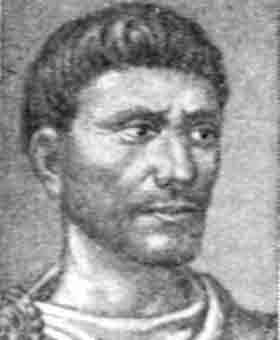
\includegraphics[width=1.5\textwidth]{diophantus.jpg}
\end{column}

\end{columns}

For instance, the equation:
$$ \dfrac{X}{Y + Z} + \dfrac{Y}{X + Z} + \dfrac{Z}{X + Y} = 4 $$
is essentially equivalent to the polynomial equation:
$$ X^3 + Y^3 + Z^3 = 3X^2Y + 3XY^2 + 3X^2Z + 3XZ^2 + 3Y^2Z + 3YZ^2 + 5XYZ $$

\vspace{0.5cm} To \textbf{solve} a Diophantine equation means to find all its \emph{integer} solutions. Are there any? Can we write one down? Are there infinitely many? Can we generate them systematically? How are they distributed?

\end{frame}

\begin{frame}[t]{Some examples}

Here are some famous Diophantine equations.
\begin{itemize}
\item Pythagoras's equation $ X^2 + Y^2 = Z^2 $. This has solutions:
$$ X = (m^2 - n^2)k \qquad Y = 2mnk \qquad Z = (m^2 + n^2)k $$
\item Pell's equation $ X^2 - nY^2 = 1 $ for fixed $ n \in \mathbb{Z} $.
\begin{itemize}
\item For $ n = 60 $, the smallest solution is $ X = 31 $ and $ Y = 4 $.
\item For $ n = 61 $, the smallest solution is $ X = 1766319049 $ and $ Y = 226153980 $.
\item For $ n = 62 $, the smallest solution is $ X = 63 $ and $ Y = 8 $.
\end{itemize}
\item Mordell's equation $ Y^2Z = X^3 - nZ^3 $ for fixed $ n \in \mathbb{Z} $.
\begin{itemize}
\item For $ n = -1 $, the only solutions are $ (-1, 0), (0, \pm1), (2, \pm3) $.
\item For $ n = 1 $, the only solutions are $ (1, 0) $.
\item For $ n = 2, 4, 11 $, there are infinitely many solutions.
\item For $ n = \pm6, \pm7 $, there are no solutions.
\end{itemize}
\item The Erd\"os--Straus conjecture says there are positive integer solutions to $ \tfrac{4}{n} = \tfrac{1}{x} + \tfrac{1}{y} + \tfrac{1}{z} $ for fixed $ n \in \mathbb{Z} $. This is still an open problem!
\end{itemize}

\end{frame}

\begin{frame}[t]{Sum of three cubes}

What $ n \in \mathbb{Z} $ can be represented as $ X^3 + Y^3 + Z^3 = n $?
\begin{itemize}
\item Does $ n = 1 $ work? Yes:
$$ 1^3 + 1^3 + (-1)^3 = 1 \qquad 9^3 + 10^3 + (-12)^3 = 1 \qquad \dots $$
\item Does $ n = 16 $ work? Yes:
$$ 2^3 + 2^3 + 0^3 = 16 \qquad (-511)^3 + (-1609)^3 + 1626^3 = 16 \qquad \dots $$
\item Do all $ n \in \mathbb{Z} $ work? No:
$$ 4, 5, 13, 14, 22, 23, 31, 32, 40, 41, 49, 50, 58, 59, 67, 68, \dots \ \text{all fail} $$
\item Does $ n = 42 $ work? Yes:
{\footnotesize $$ 12602123297335631^3 + 80435758145817515^3 + (-80538738812075974)^3 = 42 $$}%
This was only discovered in September 2019!
\item Does $ n = 114 $ work? Nobody knows as of May 2025.
\end{itemize}

\end{frame}

\begin{frame}[t]{Fermat's last theorem}

\begin{columns}[T]

\begin{column}{0.8\textwidth}
In 1637, Pierre de Fermat claimed the following theorem.

\vspace{0.5cm}

\begin{conjecture}[Fermat's last theorem]
The only integer solutions to $ X^n + Y^n = Z^n $ for some $ n > 2 $ satisfy $ XYZ = 0 $.
\end{conjecture}
\end{column}

\begin{column}{0.1\textwidth}
\hspace{-1cm}
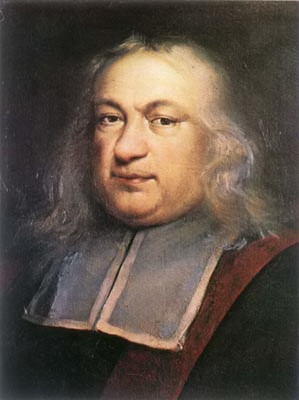
\includegraphics[width=1.5\textwidth]{fermat.jpg}
\end{column}

\end{columns}

\vspace{0.5cm} ``I have discovered a truly marvelous proof of this, which this margin is too narrow to contain.''

\vspace{0.5cm}

\begin{columns}[T]

\begin{column}{0.8\textwidth}
In 1995, Andrew Wiles published the first complete proof, which involved \emph{very advanced} 20th century mathematics.

\vspace{0.5cm} I think Fermat was mistaken.
\end{column}

\begin{column}{0.1\textwidth}
\hspace{-1cm}
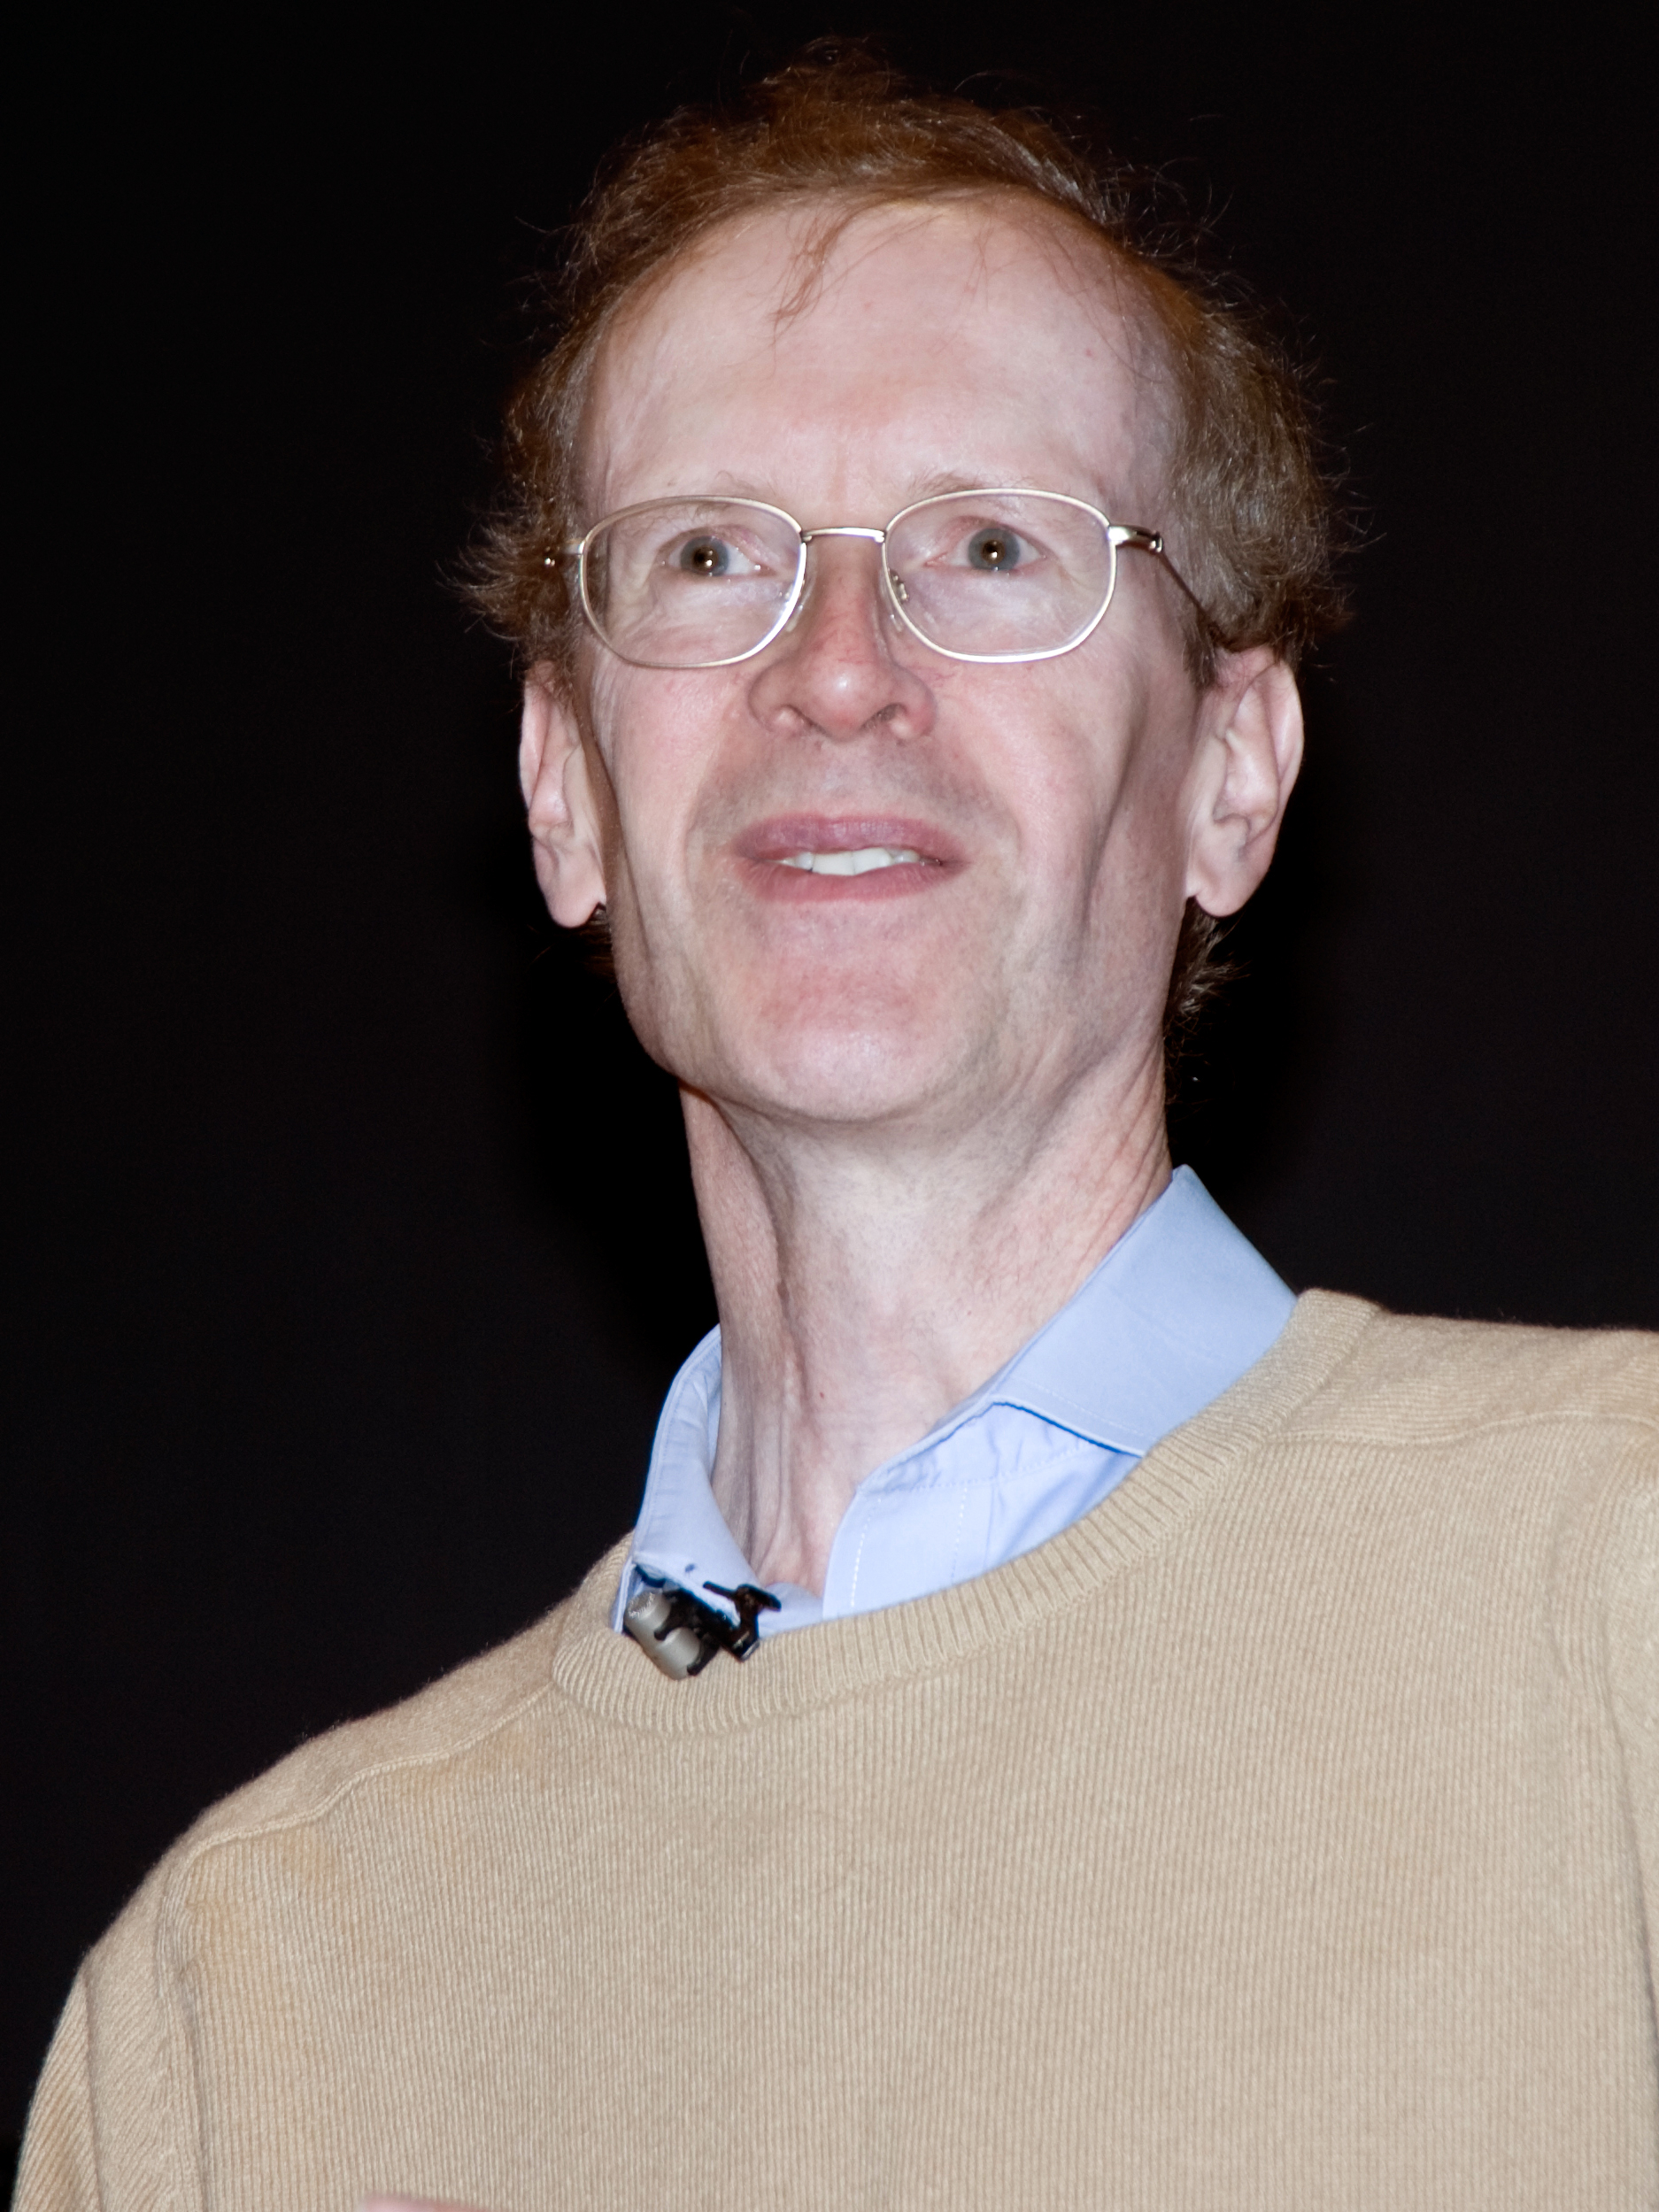
\includegraphics[width=1.5\textwidth]{wiles.jpg}
\end{column}

\end{columns}

Why are Diophantine equations so difficult?

\end{frame}

\begin{frame}[t]{Hilbert's tenth problem}

\begin{columns}[T]

\begin{column}{0.8\textwidth}
In 1900, David Hilbert published a list of 23 unsolved problems ranging over all areas of mathematics.

\vspace{0.5cm}

\begin{question}[Hilbert]
Is there an algorithm to solve \emph{any} Diophantine equation?
\end{question}
\end{column}

\begin{column}{0.1\textwidth}
\hspace{-1cm}
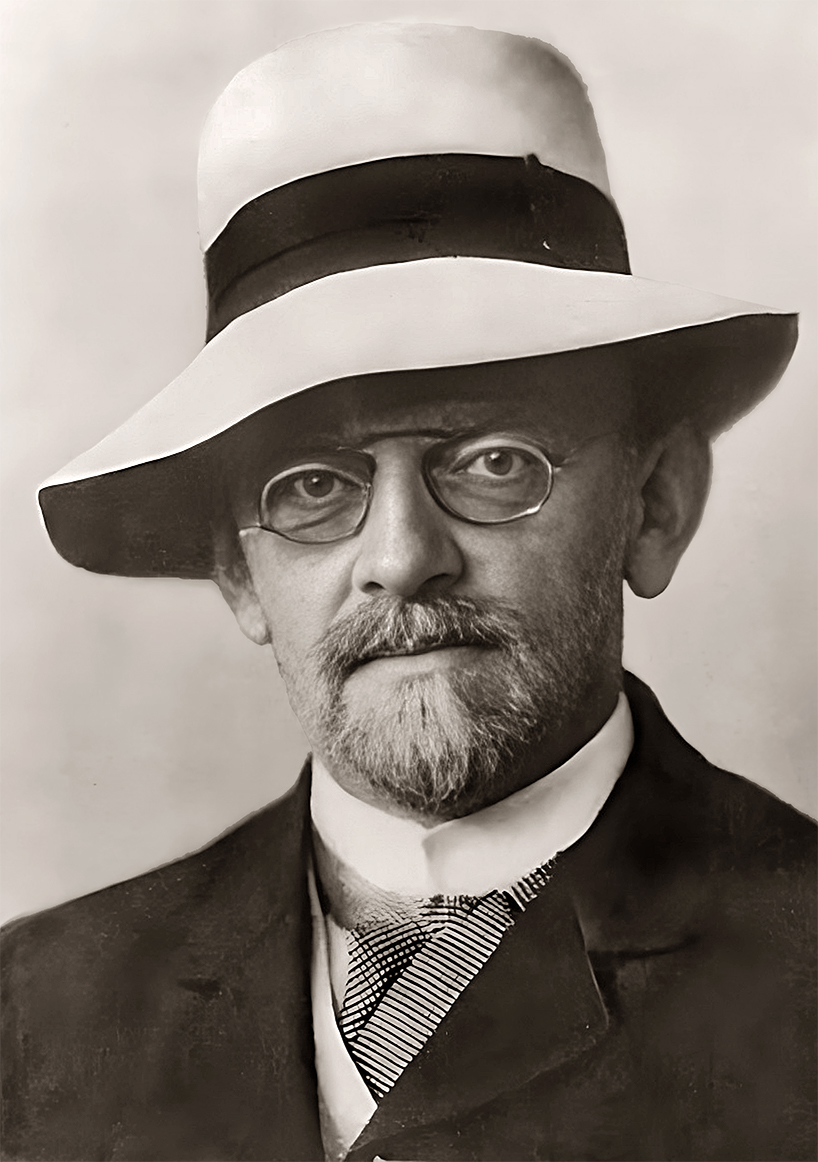
\includegraphics[width=1.5\textwidth]{hilbert.jpg}
\end{column}

\end{columns}

\vspace{0.5cm}

\begin{answer}[Davis, Matiyasevich, Putnam, Robinson]
No.
\end{answer}

\begin{center}
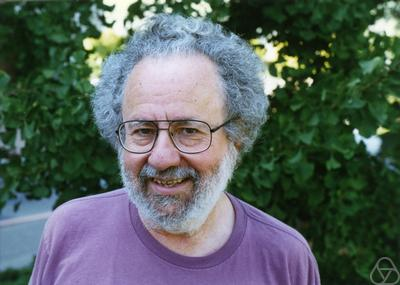
\includegraphics[width=0.2\textwidth]{davis.jpg}
\hspace{0.5cm}
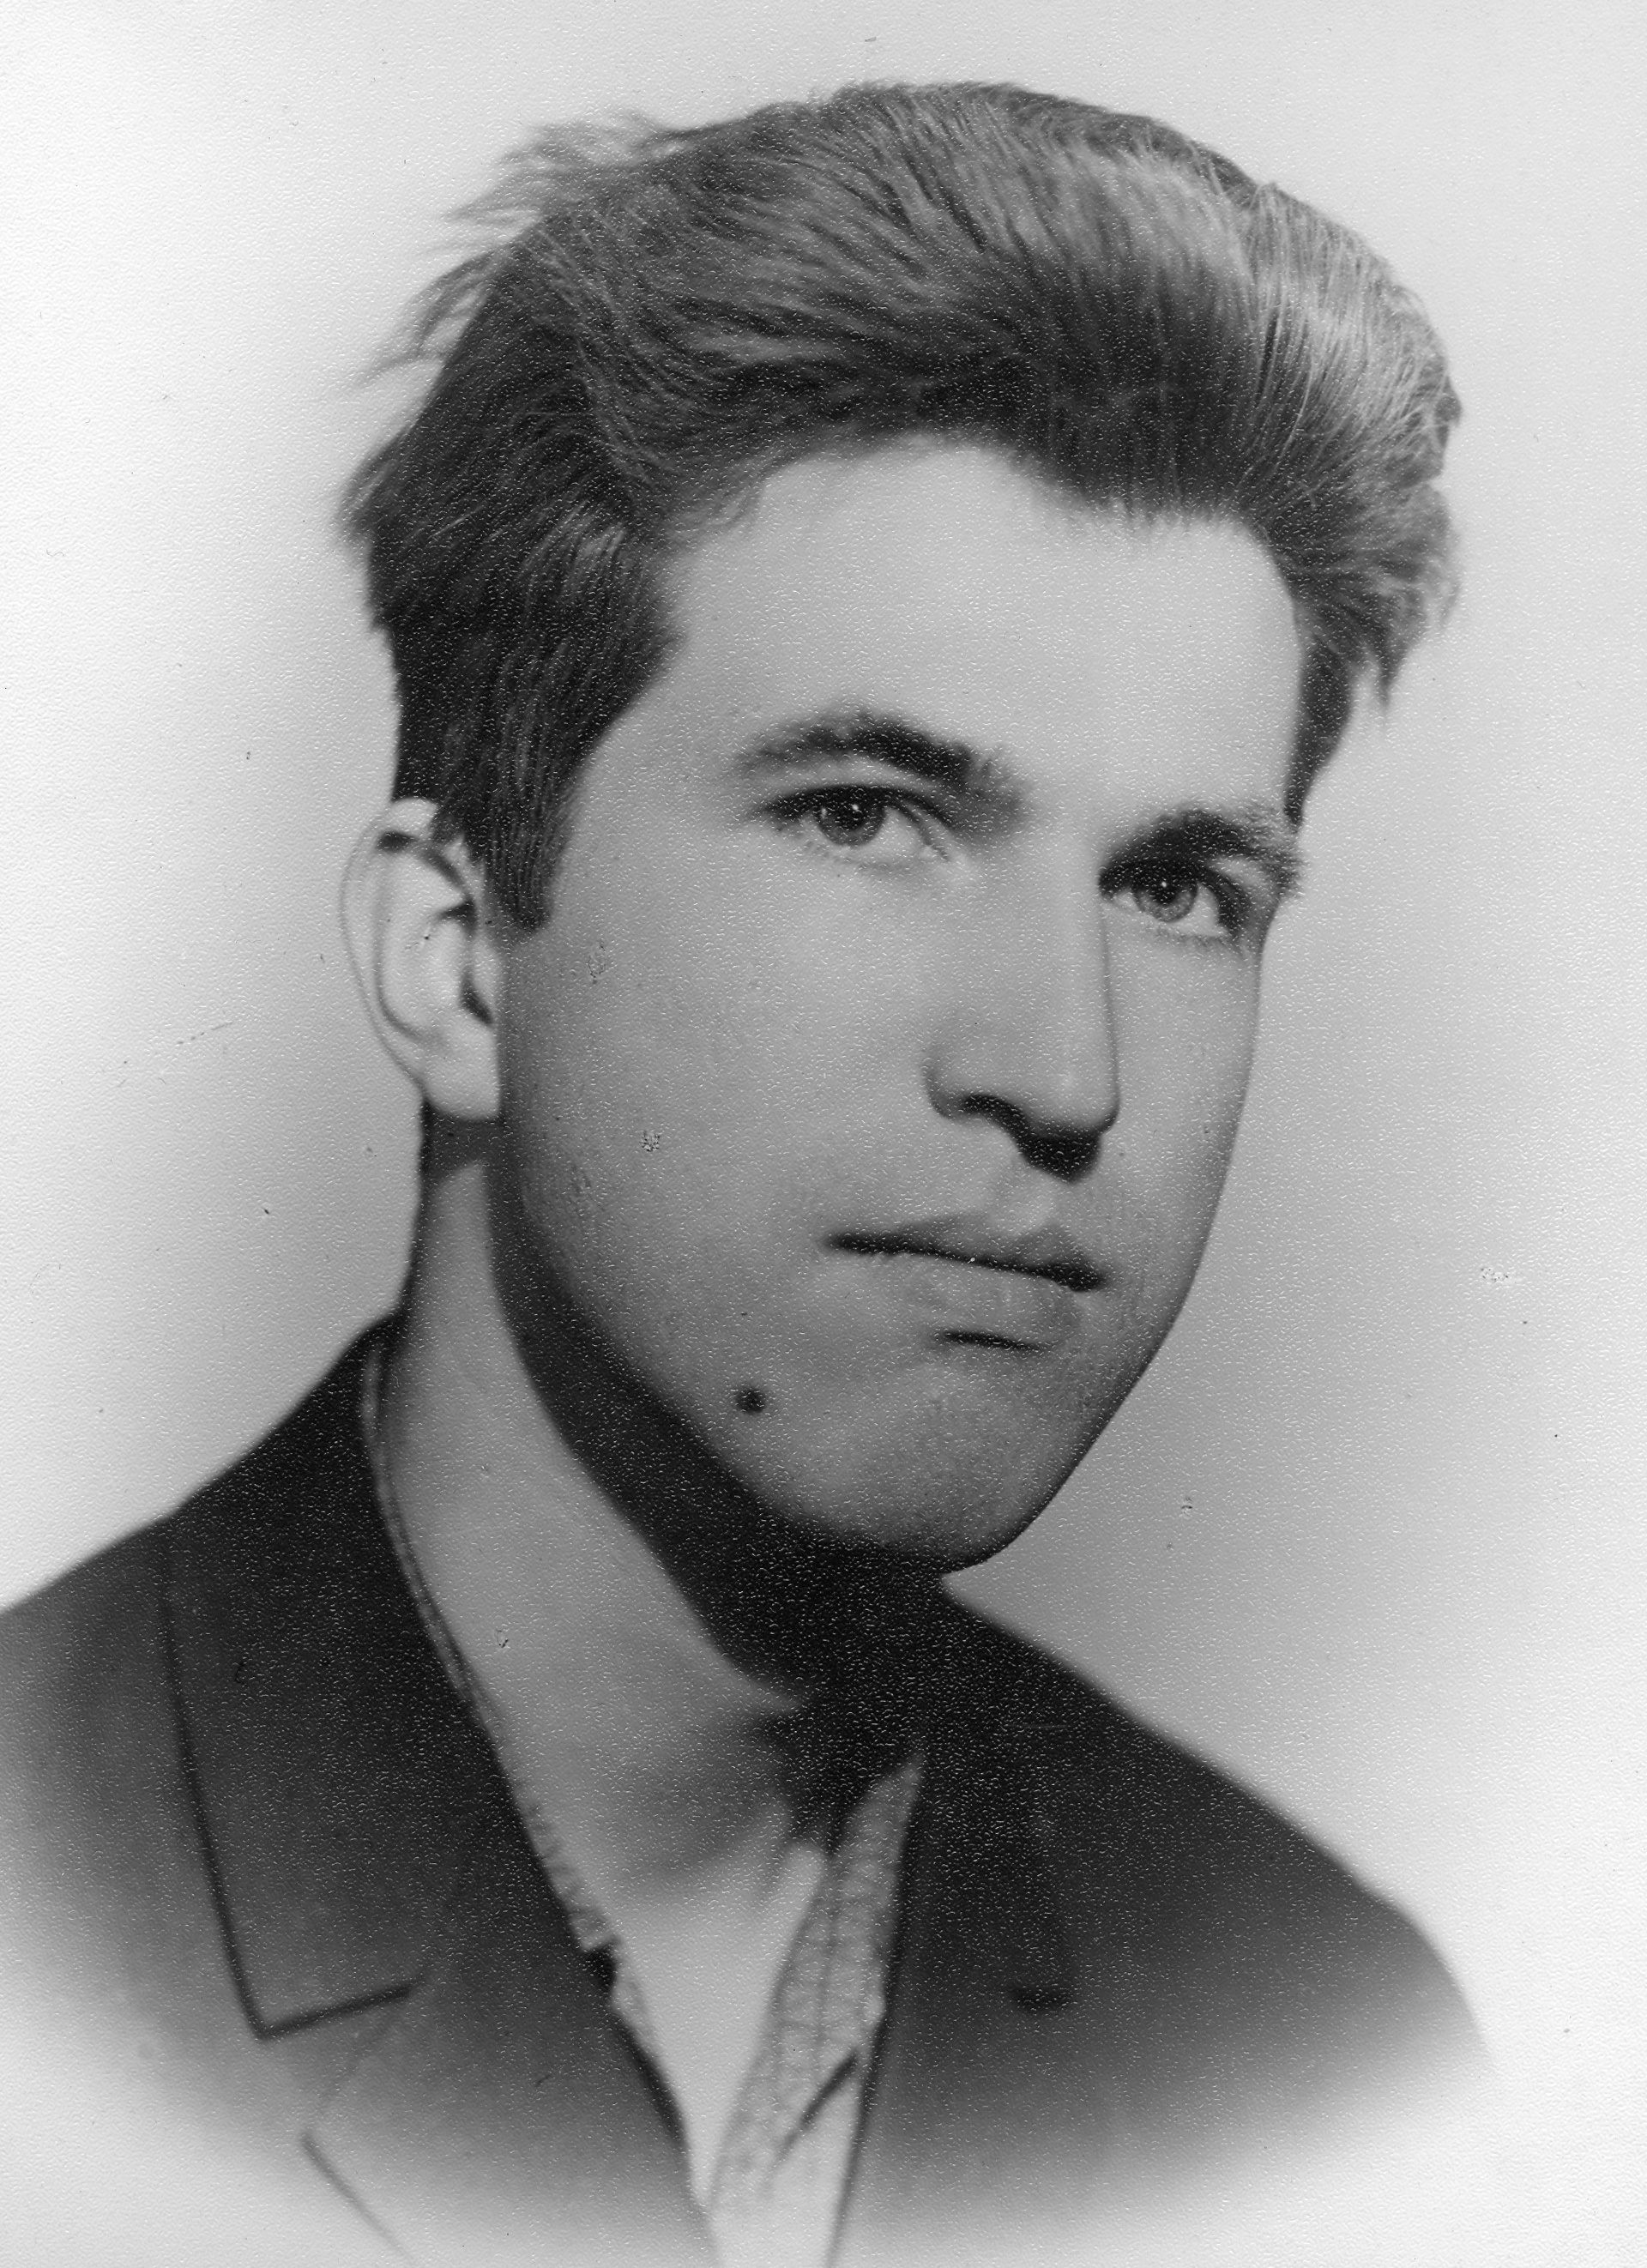
\includegraphics[width=0.1\textwidth]{matiyasevich.jpg}
\hspace{0.5cm}
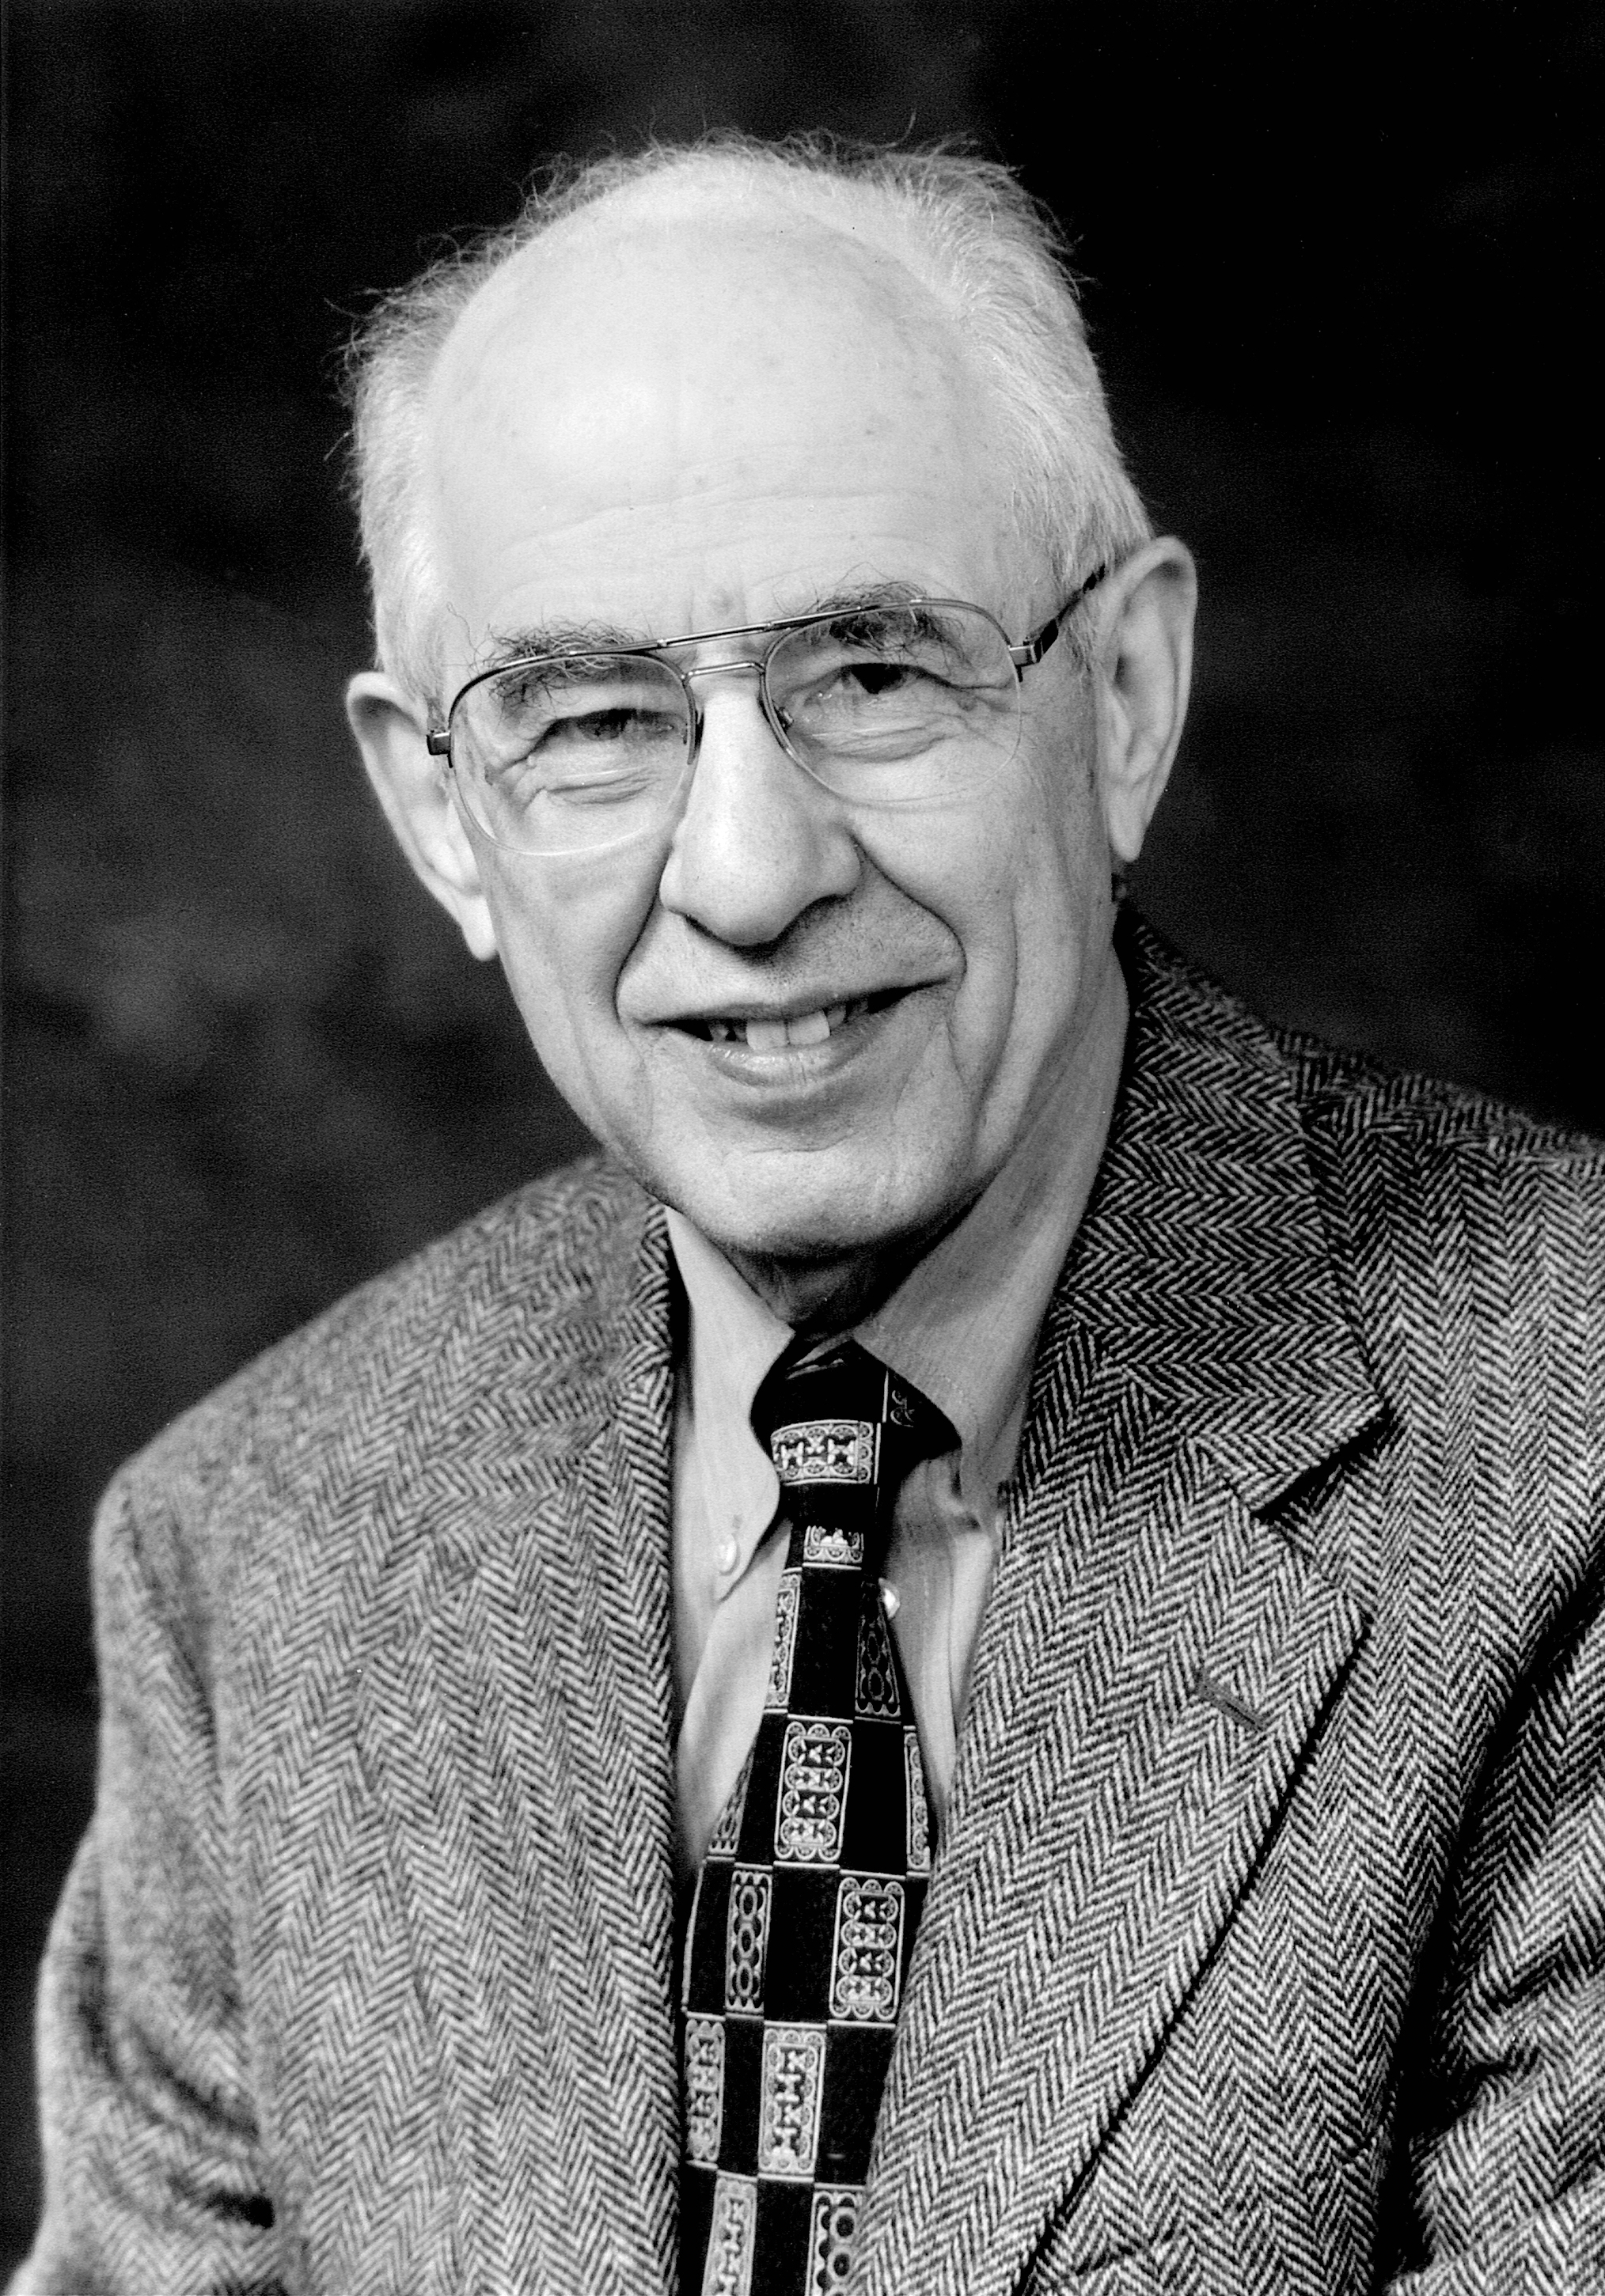
\includegraphics[width=0.1\textwidth]{putnam.jpg}
\hspace{0.5cm}
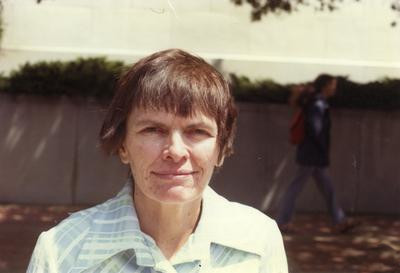
\includegraphics[width=0.2\textwidth]{robinson.jpg}
\end{center}

\vspace{0.5cm} We have to get creative!

\end{frame}

\begin{frame}[t]{Linear equations}

Observe that an integer solution gives a solution modulo $ n $ for any $ n \in \mathbb{N} $.

\vspace{0.5cm}

\begin{question}
Is there an integer solution to $ 15X + 21Y = 35 $?
\end{question}

\begin{answer}
No, because $ 15X + 21Y \equiv 0 \mod 3 $, but $ 35 \equiv 2 \mod 3 $.
\end{answer}

\vspace{0.5cm}

\begin{theorem}[B\'ezout's identity]
There is an integer solution to $ aX + bY = c $ iff $ \gcd(a, b) \mid c $. Furthermore, there is an algorithm to determine all of its solutions.
\end{theorem}

\begin{proof}
Refer to MATH0006 Algebra 2.
\end{proof}

\end{frame}

\begin{frame}[t]{B\'ezout's identity}

\begin{question}
Can we write down an integer solution to $ 15X + 21Y = 36 $?
\end{question}

\begin{answer}
Yes, because $ 36 $ is divisible by $ \gcd(15, 21) = 3 $. By the division algorithm:
\begin{align*}
21 & = 1 \cdot 15 + 6 & \text{divide $ 21 $ by $ 15 $} \\
15 & = 2 \cdot 6 + 3 & \text{divide $ 15 $ by $ 6 $}
\end{align*}
By reversing the division algorithm:
\begin{align*}
3 & = 15 - 2 \cdot 6 & \text{substitute $ 3 $} \\
& = 15 - 2 \cdot (21 - 1 \cdot 15) & \text{substitute $ 6 $} \\
& = 3 \cdot 15 - 2 \cdot 21 & \text{rearrange}
\end{align*}
Thus $ X = \tfrac{36}{3} \cdot 3 = 36 $ and $ Y = \tfrac{36}{3} \cdot -2 = -24 $ works!
\end{answer}

\end{frame}

\begin{frame}[t]{Quadratic equations}

Can we do something similar for quadratic equations $ X^2 + Y^2 = b $?

\vspace{0.5cm}

\begin{question}
Is there an integer solution to $ X^2 + Y^2 = 7^5 $?
\end{question}

\begin{answer}
No, because $ X^2, Y^2 \equiv 0, 1 \mod 4 $, but $ 7^5 \equiv 3 \mod 4 $.
\end{answer}

\vspace{0.5cm}

\begin{theorem}[Sum of two squares theorem]
There is an integer solution to $ X^2 + Y^2 = b $ iff $ b $ is not divisible by a prime congruent to $ 3 $ modulo $ 4 $ with odd exponent.
\end{theorem}

\begin{proof}
Refer to MATH0034 Number Theory.
\end{proof}

\end{frame}

\begin{frame}[t]{Sum of two squares theorem}

\begin{question}
Can we write down an integer solution to $ X^2 + Y^2 = 5^3 $?
\end{question}

\begin{answer}
Yes, because $ 5 $ is a prime congruent to $ 1 $ modulo $ 4 $. In particular, $ 5^3 $ is not divisible by any prime congruent to $ 3 $ modulo $ 4 $ with odd exponent. In the ring of Gaussian integers $ \mathbb{Z}[i] $:
$$ 5^3 = X^2 + Y^2 = (X + iY)(X - iY) $$
By \emph{unique factorisation in $ \mathbb{Z}[i] $}, write $ X \pm iY = (W \pm iZ)^3 $. Then:
$$ 5^3 = ((W + iZ)(W - iZ))^3 = (W^2 + Z^2)^3 $$
Now $ W = 2 $ and $ Z = 1 $ is an integer solution to $ W^2 + Z^2 = 5 $. Moreover:
$$ X + iY = (W + iZ)^3 = (W^3 - 3WZ^2) + i(3W^2Z - Z^3) $$
Thus $ X = W^3 - 3WZ^2 = 2 $ and $ Y = 3W^2Z - Z^3 = 11 $ works!
\end{answer}

\end{frame}

\begin{frame}[t]{Number rings}

Can we do something similar for quadratic equations $ X^2 + aY^2 = b $?

\vspace{0.5cm}

\begin{question}
Is there an integer solution to $ X^2 + 2Y^2 = 7^2 $?
\end{question}

\begin{answer}
Consider the number ring $ R := \mathbb{Z}[\sqrt{-2}] $. Factorise:
$$ 7^2 = X^2 + 2Y^2 = (X + \sqrt{-2}Y)(X - \sqrt{-2}Y) $$
\emph{By unique factorisation in $ R $}, write $ X \pm \sqrt{-2}Y = (W \pm \sqrt{-2}Z)^2 $. Then:
$$ 7^2 = ((W + \sqrt{-2}Z)(W - \sqrt{-2}Z))^2 = (W^2 + 2Z^2)^2 $$
There are no integer solutions to $ W^2 + 2Z^2 = 7 $!
\end{answer}

\vspace{0.5cm} Note that $ W^2 + 2Z^2 > 0 $, so it is easy to rule out solutions.

\end{frame}

\begin{frame}[t]{Failure of unique factorisation}

Solving the quadratic equation $ X^2 + aY^2 = b $ seems to rely on unique factorisation in the ring $ R := \mathbb{Z}[\sqrt{-a}] $, but this might fail.
\begin{examples}
\begin{itemize}
\item In $ R = \mathbb{Z}[\sqrt{-5}] $, we have $ 6 = 2 \cdot 3 = (1 + \sqrt{-5}) \cdot (1 - \sqrt{-5}) $.
\item In $ R = \mathbb{Z}[\sqrt{10}] $, we have $ 10 = 2 \cdot 5 = \sqrt{10} \cdot \sqrt{10} $.
\end{itemize}
\end{examples}
The solution is to replace $ X + \sqrt{-a} $ with the \textbf{ideal}:
$$ \langle X + \sqrt{-a}\rangle := \{(X + \sqrt{-a})r : r \in \mathbb{Z}[\sqrt{-a}]\}, $$
This has unique factorisation into \textbf{prime ideals} if $ a \not\equiv 3 \mod 4 $.

\vspace{0.5cm} The failure of unique factorisation into \emph{primes} is measured by the \textbf{ideal class group} $ \mathrm{Cl}(R) $. For some $ \mathrm{Cl}(R) $, a similar argument still works!

\vspace{0.5cm} For more details, refer to MATH0035 Algebraic Number Theory.

\end{frame}

\begin{frame}[t]{Cyclotomic rings}

\begin{columns}[T]

\begin{column}{0.8\textwidth}
In the 19th century, Ernst Kummer proved Fermat's last theorem for many exponents using this approach.

\vspace{0.5cm}

\begin{theorem}[Kummer]
If $ p $ is a regular odd prime, then the only integer solutions to $ X^p + Y^p = Z^p $ satisfy $ XYZ = 0 $.
\end{theorem}
\end{column}

\begin{column}{0.1\textwidth}
\hspace{-1cm}
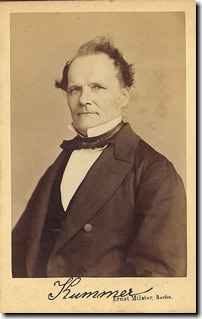
\includegraphics[width=1.5\textwidth]{kummer.jpg}
\end{column}

\end{columns}

\vspace{0.5cm} Call a prime $ p $ \textbf{regular} if it does not divide the size of $ \mathrm{Cl}(R) $.

\vspace{0.5cm} His idea was to consider the \textbf{cyclotomic ring} $ R := \mathbb{Z}[\zeta_p] $ for $ \zeta_p := e^{\frac{2\pi i}{p}} $, where a similar argument works for the factorisation:
$$ Z^p = X^p + Y^p = (X + Y) \cdot (X + \zeta_pY) \cdot (X + \zeta_p^2Y) \cdot \dots \cdot (X + \zeta_p^{p - 1}Y) $$

\vspace{0.5cm} Conjecturally, about 61\% of all primes are regular.

\end{frame}

\begin{frame}[t]{Rational projective plane}

Observe that $ X^n + Y^n = Z^n $ is \textbf{homogeneous} of degree $ n $.

\vspace{0.5cm} In particular, this \emph{almost} gives a correspondence:
$$
\begin{array}{rcl}
\{(X, Y, Z) \in \mathbb{Z}^3 : X^n + Y^n = Z^n\} & \leftrightsquigarrow & \{(x, y) \in \mathbb{Q}^2 : x^n + y^n = 1\} \\
(X, Y, Z) & \mapsto & (\tfrac{X}{Z}, \tfrac{Y}{Z}) \\
(xz, yw, wz) & \mapsfrom & (\tfrac{x}{w}, \tfrac{y}{z})
\end{array}
$$
This correspondence is not quite bijective:
\begin{itemize}
\item Both $ (X, Y, Z) $ and $ (\lambda X, \lambda Y, \lambda Z) $ map to $ (\tfrac{X}{Z}, \tfrac{Y}{Z}) $.
\item Where does $ (X, Y, 0) $ map to?
\end{itemize}
Both of these issues can be fixed by working in the \textbf{projective plane}.
\begin{itemize}
\item Replace the left hand side with equivalence classes up to scaling.
\item Supplement the right hand side with ``points at infinity''.
\end{itemize}

\vspace{0.5cm} For more details, refer to MATH0076 Algebraic Geometry.

\end{frame}

\begin{frame}[t]{Fermat curves}

By working in the projective plane:
$$ \left\{\begin{array}{c} \text{\emph{integer} solutions of} \\ X^n + Y^n = Z^n \end{array}\right\} \leftrightsquigarrow \left\{\begin{array}{c} \text{\emph{rational} solutions of} \\ x^n + y^n = 1 \end{array}\right\} $$

\vspace{0.5cm}

\begin{columns}[T]

\begin{column}{0.7\textwidth}
When $ n = 3 $, the cubic equation $ x^3 + y^3 = 1 $ defines an object in algebraic geometry called an \textbf{elliptic curve}, which lives in the projective plane.

\vspace{0.5cm} In particular, rational solutions of the equation correspond to \textbf{rational points} on the curve.
\end{column}

\begin{column}{0.2\textwidth}
\hspace{-1cm}
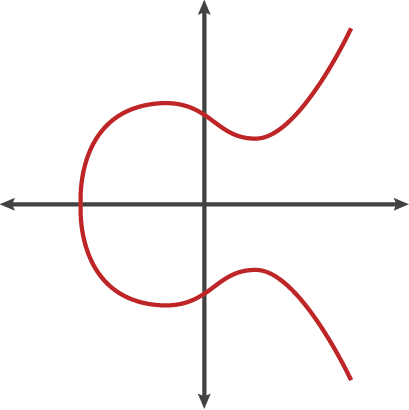
\includegraphics[width=1.2\textwidth]{ellipticcurve.png}
\end{column}

\end{columns}

\vspace{0.5cm} In fact, the fruit equation
$$ X^3 + Y^3 + Z^3 = 3X^2Y + 3XY^2 + 3X^2Z + 3XZ^2 + 3Y^2Z + 3YZ^2 + 5XYZ $$
also defines an elliptic curve!

\end{frame}

\begin{frame}[t]{Elliptic curves}

The set of rational points on an elliptic curve forms an abelian group:
$$ P + Q + R = 0 \qquad \iff \qquad P, Q, R \ \text{are collinear} $$

\begin{center}
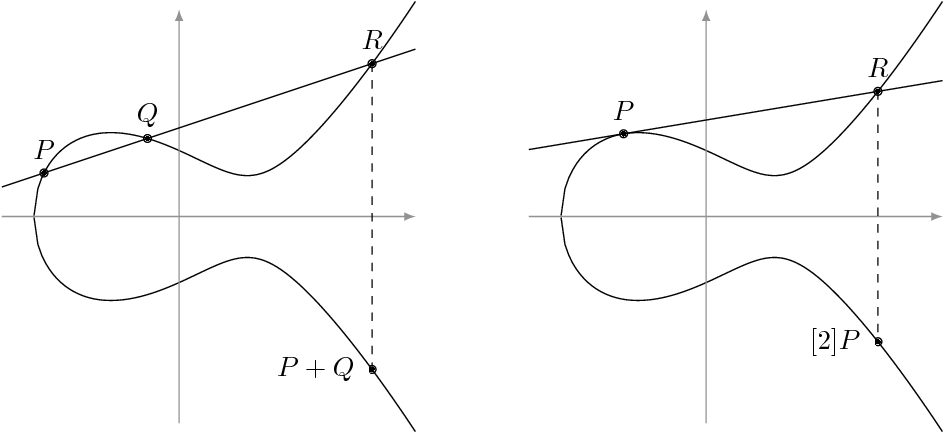
\includegraphics[width=0.9\textwidth]{grouplaw.png}
\end{center}

This gives a way to generate new rational solutions from old ones!

\end{frame}

\begin{frame}[t]{Cubic equations}

\begin{question}
Can we write down two rational solutions to $ x^3 - y^2 = 4 $?
\end{question}

\begin{answer}
This defines an elliptic curve, with a rational solution $ x = 2 $ and $ y = 2 $. The tangent of $ e(x, y) = x^3 - y^2 - 4 $ at the rational point $ (2, 2) $ is:
$$ \dfrac{\partial e}{\partial x}(2) \cdot (x - 2) + \dfrac{\partial e}{\partial y}(2) \cdot (y - 2) = 0 $$
This simplifies as $ y = 3x - 4 $, which substitutes into $ e(x, y) = 0 $ to yield:
$$ 0 = x^3 - (3x - 4)^2 - 4 = (x - 2)^2(x - 5) $$
Thus $ y = 3(5) - 4 = 11 $, so $ (5, 11) $ works!
\end{answer}

\vspace{0.5cm} In fact, \emph{adding} the rational point $ (2, 2) $ to itself repeatedly generates the \emph{only} infinite family of rational solutions to $ x^3 - y^2 = 4 $.

\end{frame}

\begin{frame}[t]{Mordell's theorem}

\begin{columns}[T]

\begin{column}{0.8\textwidth}
In 1922, Louis Mordell classified the abstract group structure of rational points on elliptic curves.

\vspace{0.5cm}

\begin{theorem}[Mordell]
The rational points on an elliptic curve can be generated from a finite set of initial rational points.
\end{theorem}
\end{column}

\begin{column}{0.1\textwidth}
\hspace{-1cm}
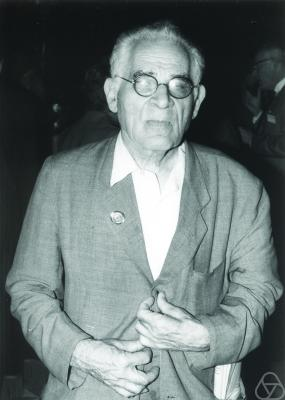
\includegraphics[width=1.5\textwidth]{mordell.jpg}
\end{column}

\end{columns}

\vspace{0.5cm} Associated to an elliptic curve $ E $ is a complex-analytic \textbf{L-function} $ L_E(s) $.

\begin{conjecture}[Birch, Swinnerton-Dyer]
An elliptic curve $ E $ has infinitely many rational points iff $ L_E(1) = 0 $.
\end{conjecture}

\begin{center}
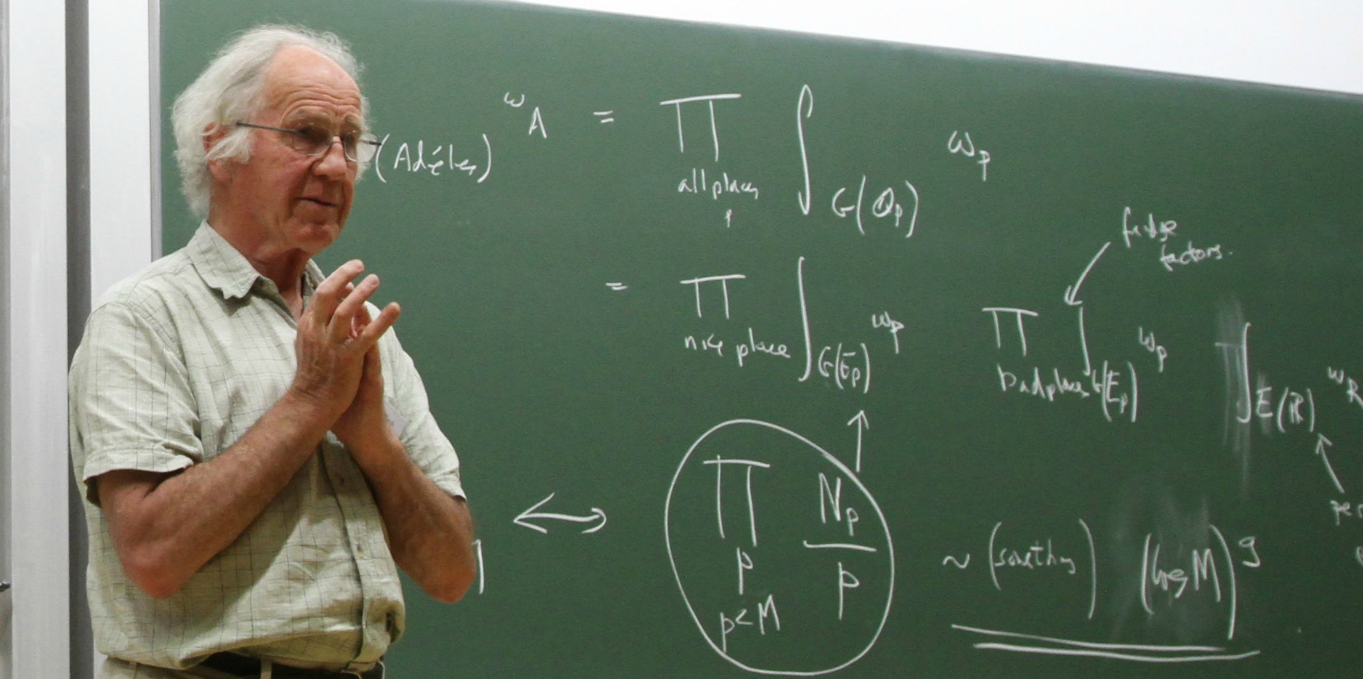
\includegraphics[width=0.2\textwidth]{birch.jpg}
\hspace{0.5cm}
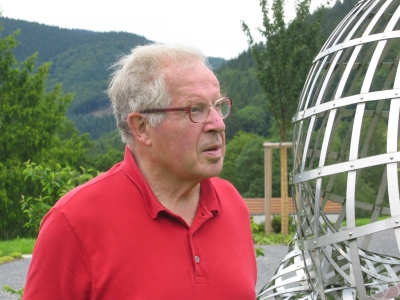
\includegraphics[width=0.15\textwidth]{swinnertondyer.jpg}
\end{center}
For more details, refer to MATH0036 Elliptic Curves.

\end{frame}

\begin{frame}[t]{Modular forms}

\begin{columns}[T]

\begin{column}{0.7\textwidth}
Andrew Wiles proved Fermat's last theorem by studying properties of general L-functions.

\vspace{0.5cm} Another object with an associated L-function is a \textbf{modular form}, which is a highly symmetric function on the upper half $ \mathcal{H} $ of the complex plane.
\end{column}

\begin{column}{0.2\textwidth}
\hspace{-1cm}
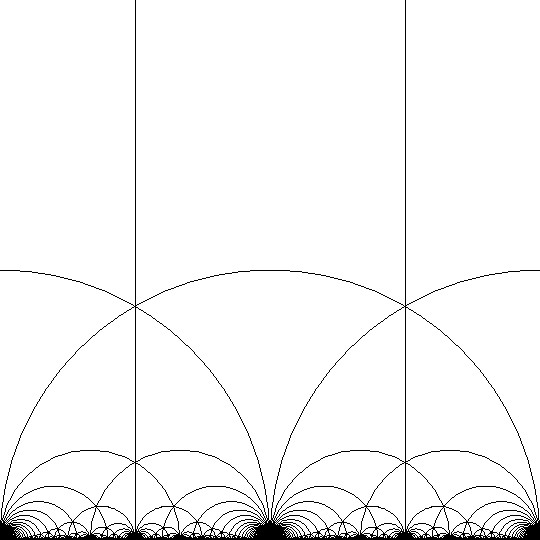
\includegraphics[width=1.2\textwidth]{modularform.jpg}
\end{column}

\end{columns}

\vspace{0.5cm}

\begin{conjecture}[Shimura, Taniyama, Weil]
Elliptic curves are related to modular forms.
\end{conjecture}

\begin{center}
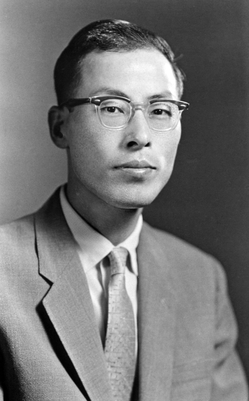
\includegraphics[width=0.12\textwidth]{shimura.jpg}
\hspace{0.5cm}

\includegraphics[width=0.12\textwidth]{taniyama.jpg}
\hspace{0.5cm}
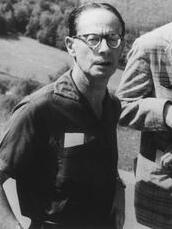
\includegraphics[width=0.15\textwidth]{weil.jpg}
\end{center}

\end{frame}

\begin{frame}[t]{Newforms}

The modular forms of interest are the so-called \textbf{level-$ N $ newforms}.

\vspace{0.5cm} These are functions $ f : \mathcal{H} \to \mathbb{C} $ satisfying the \textbf{modular condition}:
$$ f\left(\dfrac{az + b}{cz + d}\right) = (cz + d)^2 \cdot f(z) $$
for any $ a, b, c, d \in \mathbb{Z} $ such that $ ad - bc = 1 $ and $ N \mid c $.

\vspace{0.5cm}

\begin{theorem}[Valence formula]
For fixed $ N $, there are finitely many level-$ N $ newforms.
\end{theorem}

\vspace{0.5cm} In fact, there are \emph{no} level-$ N $ newforms for:
$$ N \in \{1, 2, 3, 4, 5, 6, 7, 8, 9, 10, 12, 13, 16, 18, 22, 25, 28, 60\} $$
For more details, refer to MATH0104 Modular Forms.

\end{frame}

\begin{frame}[t]{Modularity theorem}

Also associated to a modular form $ f $ is its \textbf{Hecke L-function} $ L_f(s) $.

\vspace{0.5cm}

\begin{columns}[T]

\begin{column}{0.8\textwidth}
Call an elliptic curve $ E $ \textbf{modular} if there is a level-$ N $ newform $ f $ such that $ L_E(s) = L_f(s) $ for some $ N $.

\vspace{0.5cm}

\begin{theorem}[Wiles]
For squarefree $ N $, all elliptic curves are modular.
\end{theorem}
\end{column}

\begin{column}{0.1\textwidth}
\hspace{-1cm}
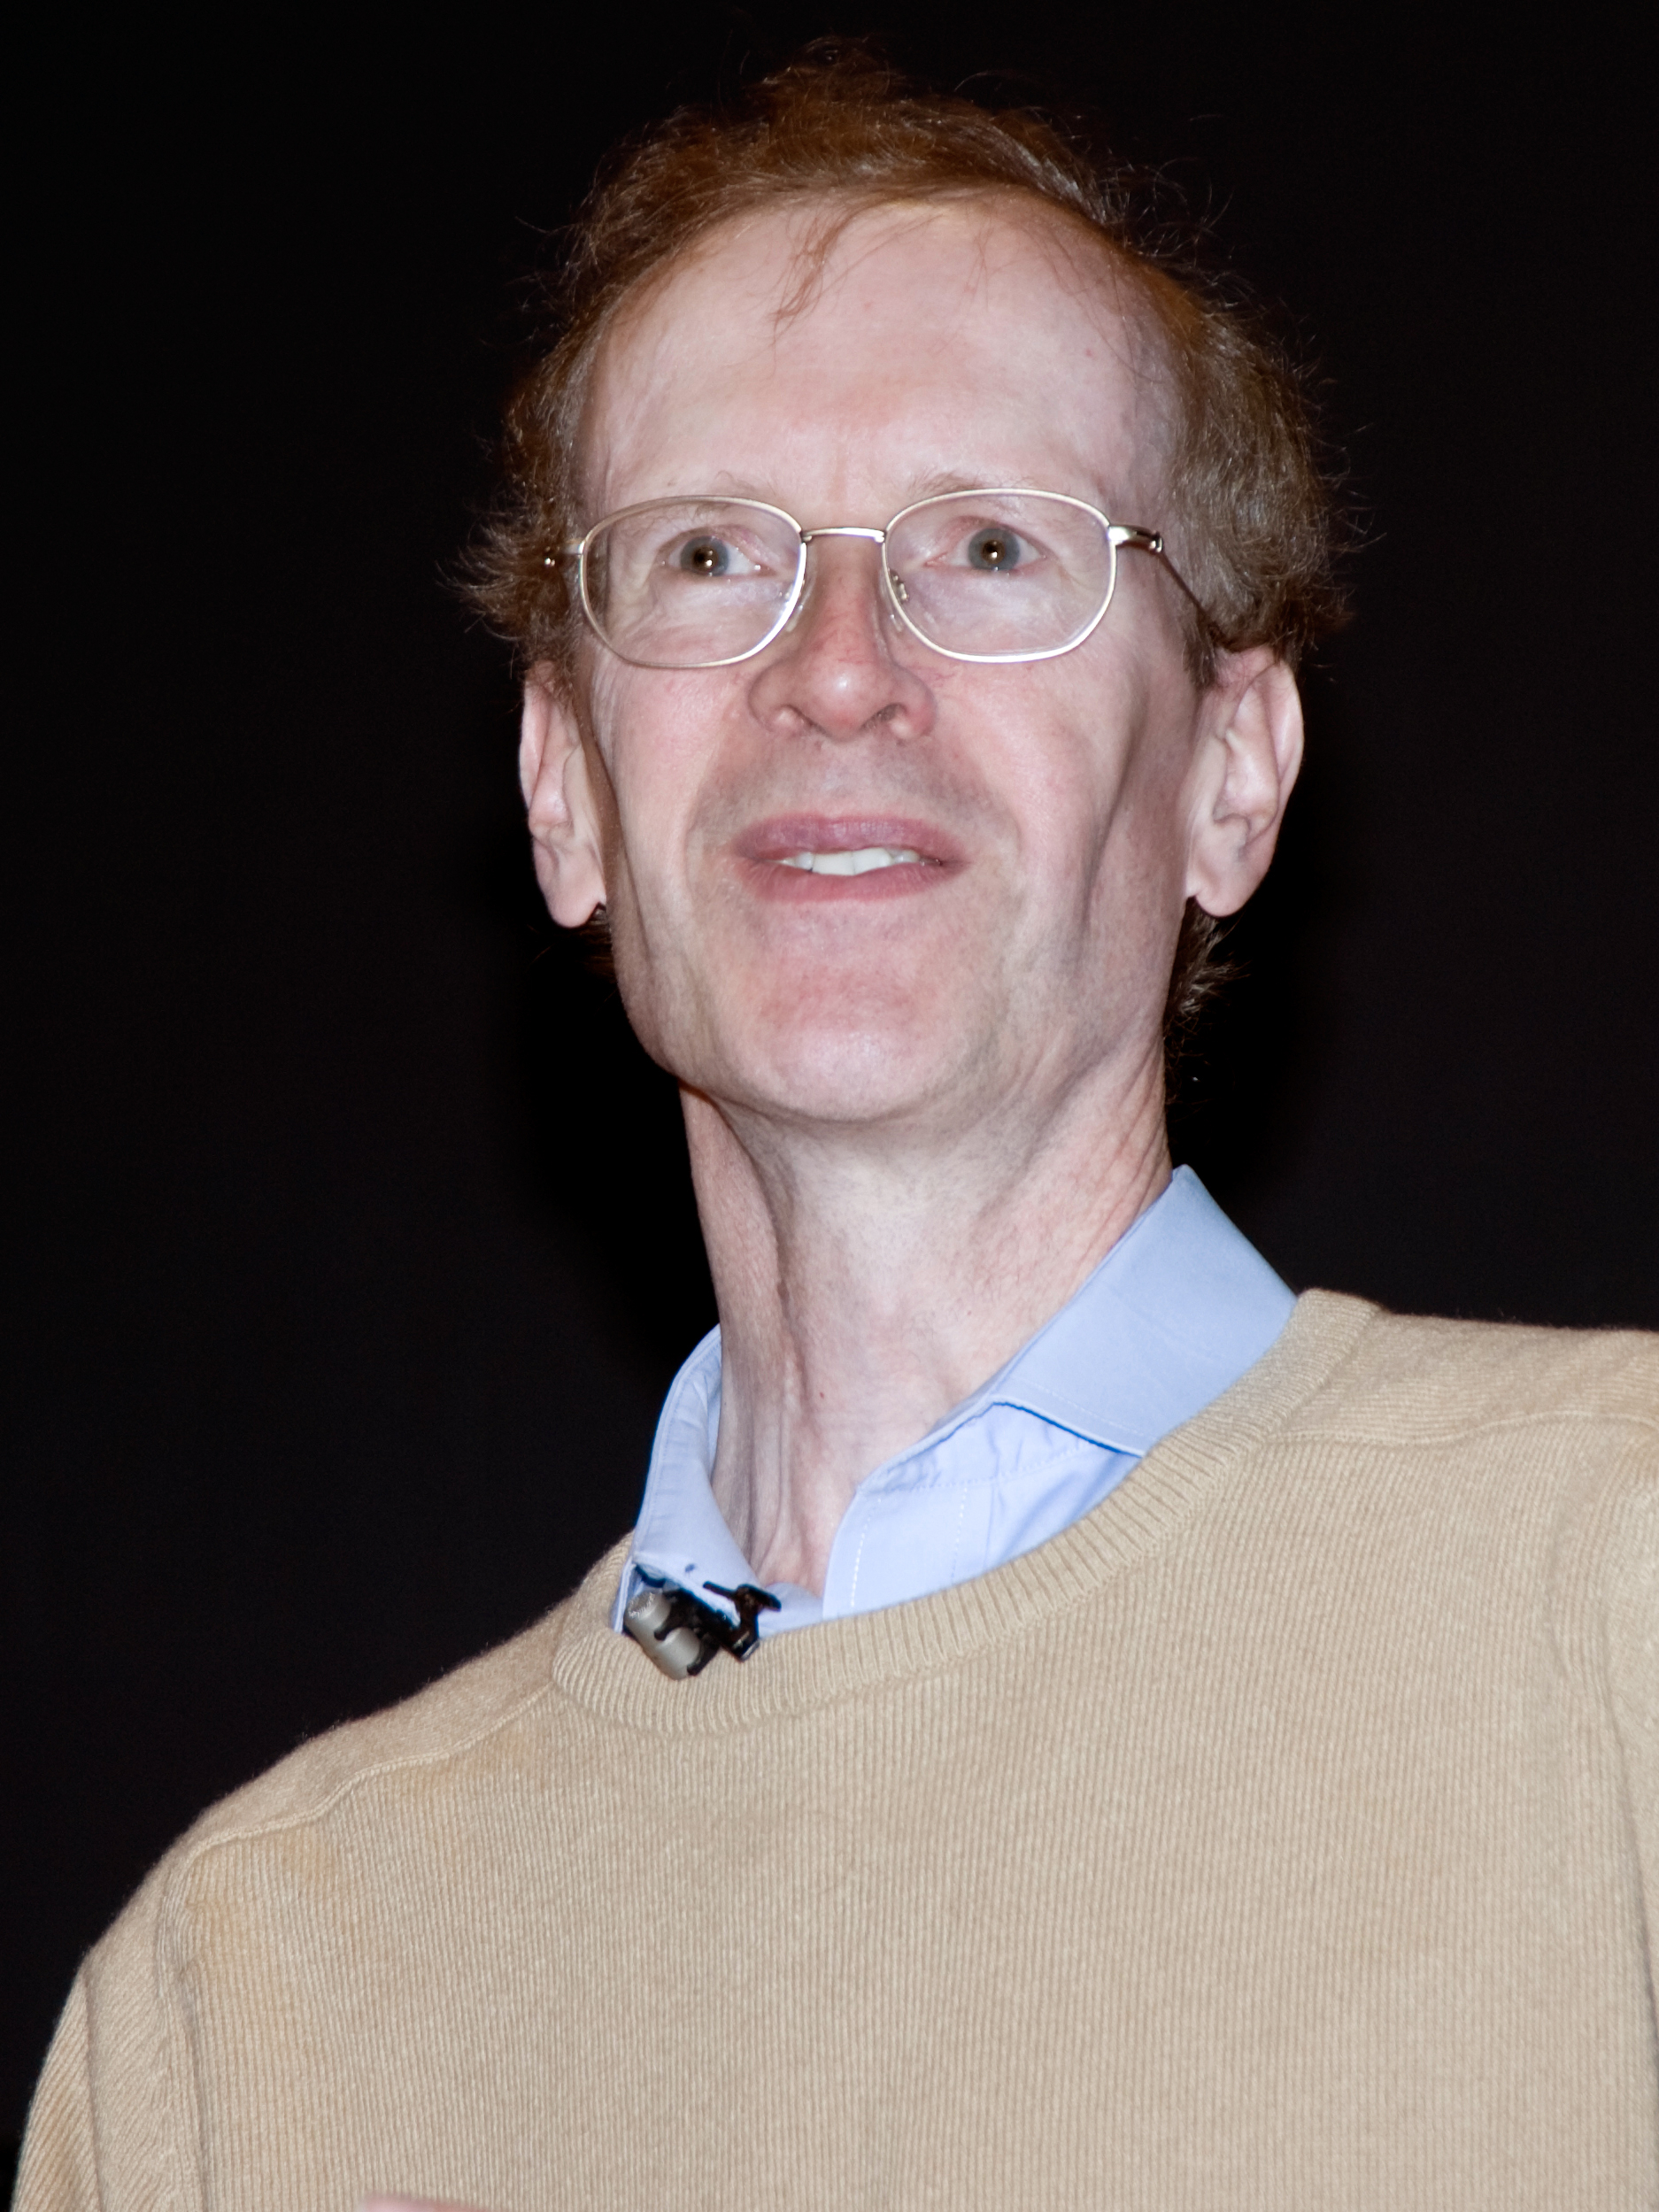
\includegraphics[width=1.5\textwidth]{wiles.jpg}
\end{column}

\end{columns}

\vspace{0.5cm}

\begin{theorem}[Breuil, Conrad, Diamond, Taylor]
All elliptic curves are modular.
\end{theorem}

\begin{center}
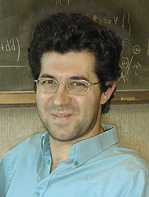
\includegraphics[width=0.1\textwidth]{breuil.jpg}
\hspace{0.5cm}
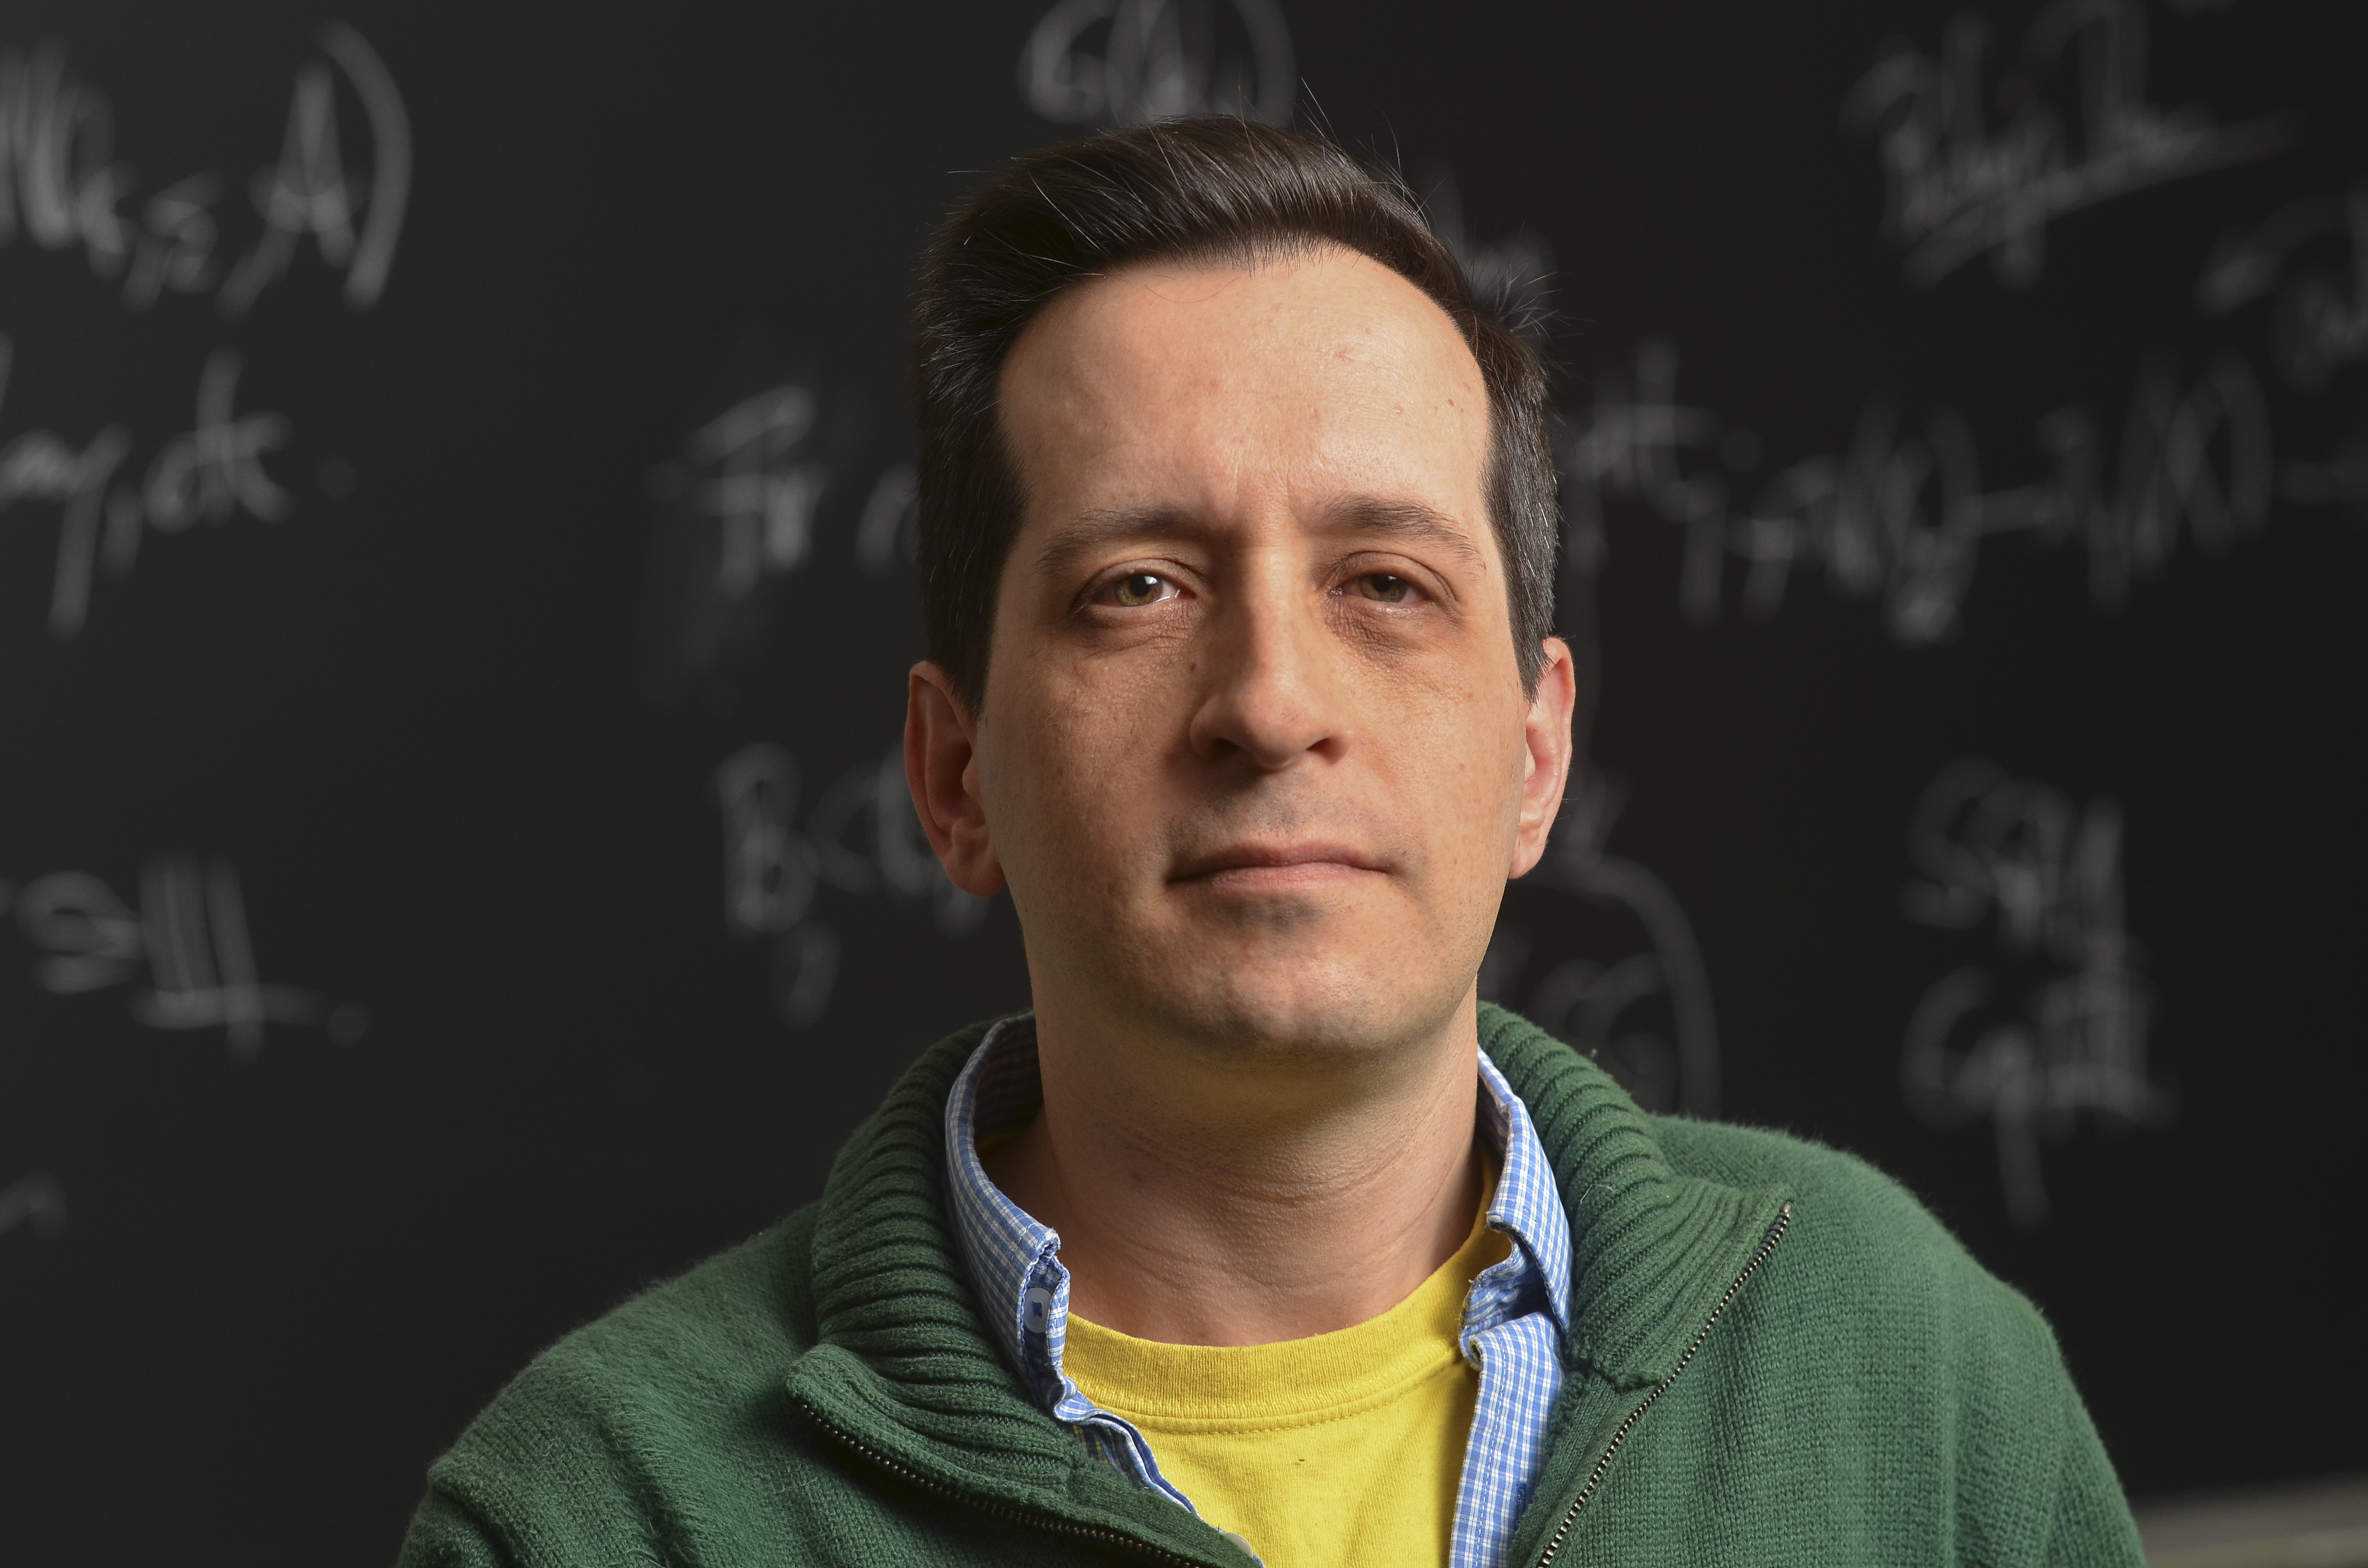
\includegraphics[width=0.2\textwidth]{conrad.jpg}
\hspace{0.5cm}
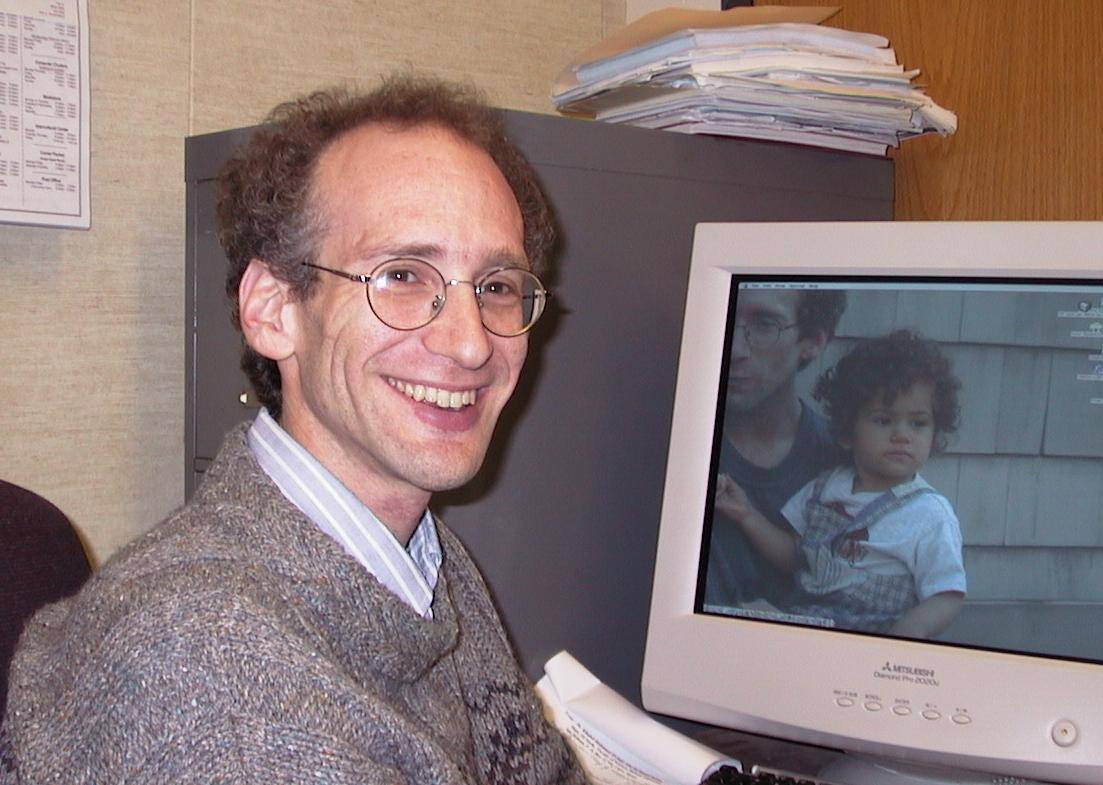
\includegraphics[width=0.2\textwidth]{diamond.jpg}
\hspace{0.5cm}
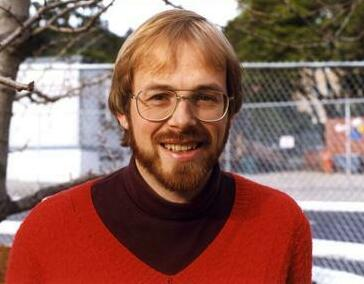
\includegraphics[width=0.2\textwidth]{taylor.jpg}
\end{center}

\end{frame}

\begin{frame}[t]{Fermat's last theorem}

Fermat's last theorem can now be deduced from the modularity theorem.

\vspace{0.5cm} Assume for a contradiction that $ X^n + Y^n = Z^n $ has an integer solution not satisfying $ XYZ = 0 $. Consider the elliptic curve $ E $ given by:
$$ y^2 = x(x - X^n)(x + Y^n) $$
This is called the \textbf{Frey curve} associated to the triple $ (X, Y, Z) $.

\vspace{0.5cm} The modularity theorem says that $ E $ corresponds to a level-$ N $ newform $ f $.

\begin{columns}[T]

\begin{column}{0.8\textwidth}
\vspace{0.5cm}

\begin{theorem}[Ribet]
$ f $ can be ``level-lowered'' to a level-$ 2 $ newform.
\end{theorem}

\vspace{0.5cm} There are no level-$ 2 $ newforms, hence a contradiction!
\end{column}

\begin{column}{0.1\textwidth}
\begin{center}
\hspace{-1cm}
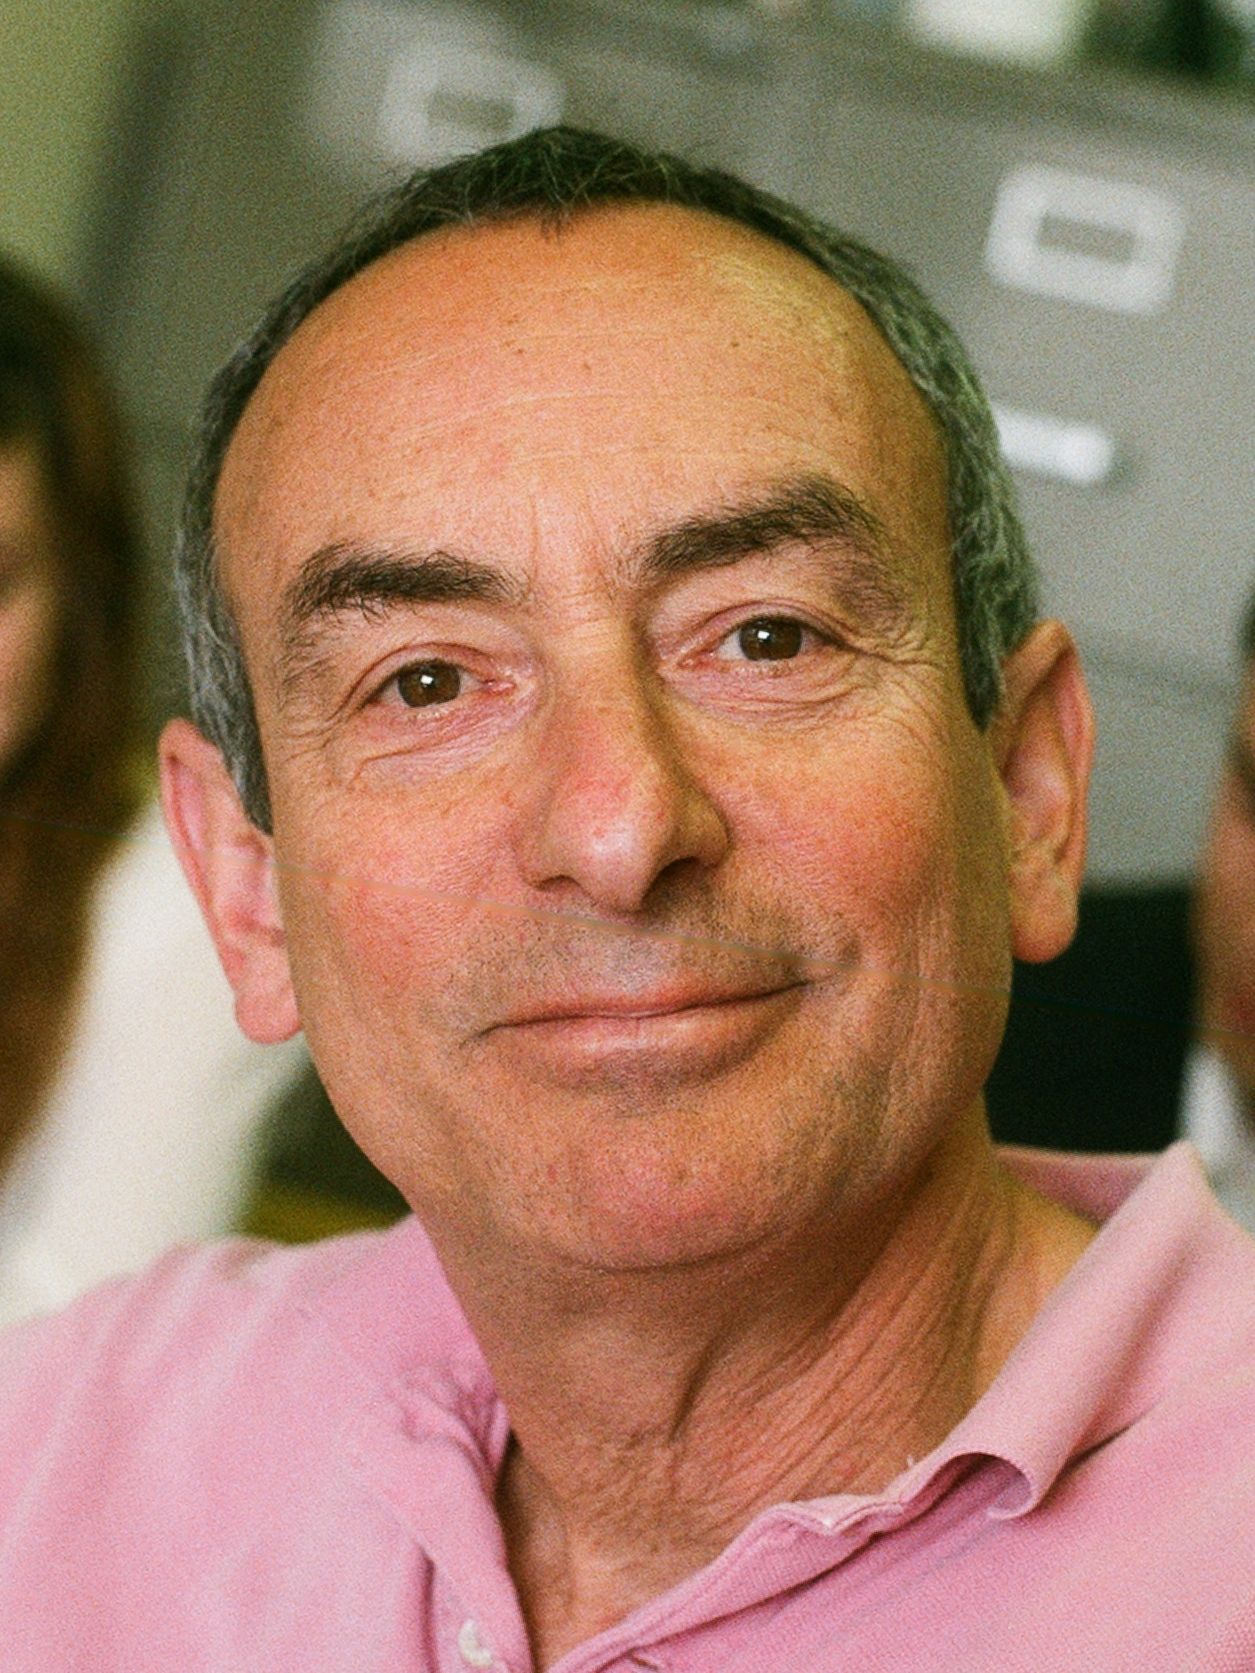
\includegraphics[width=1.5\textwidth]{ribet.jpg}
\end{center}
\end{column}

\end{columns}

\end{frame}

\begin{frame}[t]{Formalising Fermat}

\begin{columns}[T]

\begin{column}{0.8\textwidth}
My PhD supervisor Kevin Buzzard started a massive project to teach the modularity theorem to a computer.
\end{column}

\begin{column}{0.1\textwidth}
\begin{center}
\vspace{-1cm}
\hspace{-1cm}

\includegraphics[width=1.5\textwidth]{buzzard.jpg}
\end{center}
\end{column}

\end{columns}

\vspace{0.5cm} This means \emph{formally} defining all the relevant objects (elliptic curves, modular forms) and \emph{rigorously} verifying all the details of the proof.

\vspace{0.5cm}

\begin{center}
\texttt{https://imperialcollegelondon.github.io/FLT/}
\end{center}

\vspace{0.5cm} This is a \emph{huge} amount of work, and we need \emph{all} the help we can get!

\vspace{0.5cm} To get started, check out MATH0109 Theorem Proving in Lean!

\begin{center}
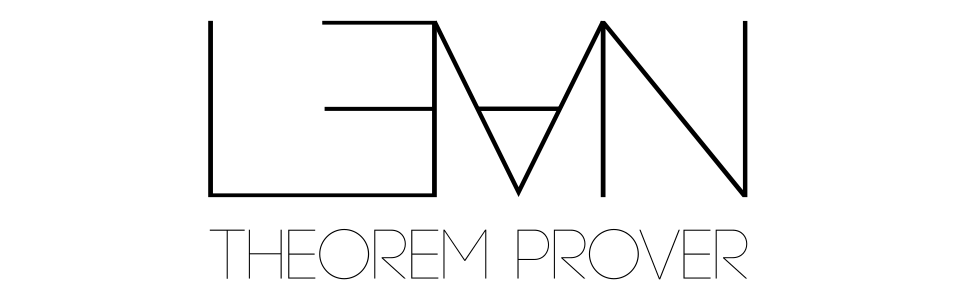
\includegraphics[width=0.5\textwidth]{lean.png}
\end{center}

\end{frame}

\end{document}